\documentclass[10pt]{article}
\usepackage{tikz}
\usetikzlibrary{shapes.misc}
\usepackage[margin=0cm]{geometry}
\pagestyle{empty}
\tikzstyle{every node}=[cross out, draw, red]

\begin{document}

\vspace*{\fill}
\begin{center}
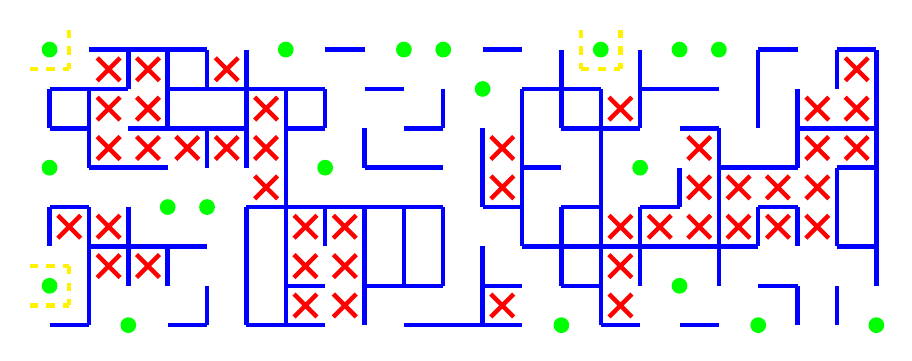
\begin{tikzpicture}[x=0.5cm, y=-0.5cm, ultra thick, blue]
% Walls
    \draw (1,0) -- (4,0);
    \draw (7,0) -- (8,0);
    \draw (11,0) -- (12,0);
    \draw (18,0) -- (19,0);
    \draw (20,0) -- (21,0);
    \draw (0,1) -- (2,1);
    \draw (3,1) -- (7,1);
    \draw (8,1) -- (9,1);
    \draw (12,1) -- (14,1);
    \draw (15,1) -- (17,1);
    \draw (0,2) -- (1,2);
    \draw (2,2) -- (5,2);
    \draw (6,2) -- (7,2);
    \draw (9,2) -- (10,2);
    \draw (13,2) -- (15,2);
    \draw (16,2) -- (17,2);
    \draw (19,2) -- (21,2);
    \draw (1,3) -- (3,3);
    \draw (8,3) -- (10,3);
    \draw (12,3) -- (13,3);
    \draw (17,3) -- (19,3);
    \draw (20,3) -- (21,3);
    \draw (0,4) -- (1,4);
    \draw (5,4) -- (10,4);
    \draw (11,4) -- (12,4);
    \draw (13,4) -- (14,4);
    \draw (15,4) -- (16,4);
    \draw (18,4) -- (19,4);
    \draw (1,5) -- (4,5);
    \draw (12,5) -- (18,5);
    \draw (20,5) -- (21,5);
    \draw (6,6) -- (7,6);
    \draw (8,6) -- (10,6);
    \draw (11,6) -- (12,6);
    \draw (13,6) -- (14,6);
    \draw (18,6) -- (19,6);
    \draw (0,7) -- (1,7);
    \draw (3,7) -- (4,7);
    \draw (5,7) -- (7,7);
    \draw (9,7) -- (12,7);
    \draw (14,7) -- (15,7);
    \draw (16,7) -- (17,7);
    \draw (0,1) -- (0,2);
    \draw (0,4) -- (0,5);
    \draw (1,1) -- (1,3);
    \draw (1,4) -- (1,7);
    \draw (2,0) -- (2,1);
    \draw (2,4) -- (2,6);
    \draw (3,0) -- (3,2);
    \draw (3,5) -- (3,6);
    \draw (4,0) -- (4,1);
    \draw (4,2) -- (4,3);
    \draw (4,6) -- (4,7);
    \draw (5,0) -- (5,3);
    \draw (5,4) -- (5,7);
    \draw (6,1) -- (6,7);
    \draw (7,1) -- (7,2);
    \draw (7,4) -- (7,5);
    \draw (8,2) -- (8,3);
    \draw (8,4) -- (8,7);
    \draw (9,4) -- (9,6);
    \draw (10,1) -- (10,2);
    \draw (10,4) -- (10,6);
    \draw (11,2) -- (11,4);
    \draw (11,5) -- (11,7);
    \draw (12,1) -- (12,5);
    \draw (13,0) -- (13,2);
    \draw (13,4) -- (13,6);
    \draw (14,1) -- (14,7);
    \draw (15,0) -- (15,2);
    \draw (15,4) -- (15,6);
    \draw (16,3) -- (16,4);
    \draw (17,2) -- (17,6);
    \draw (18,0) -- (18,2);
    \draw (18,4) -- (18,5);
    \draw (19,1) -- (19,3);
    \draw (19,4) -- (19,5);
    \draw (19,6) -- (19,7);
    \draw (20,0) -- (20,1);
    \draw (20,3) -- (20,5);
    \draw (20,6) -- (20,7);
    \draw (21,0) -- (21,6);
% Pillars
    \fill[green] (0,0) circle(0.2);
    \fill[green] (6,0) circle(0.2);
    \fill[green] (9,0) circle(0.2);
    \fill[green] (10,0) circle(0.2);
    \fill[green] (14,0) circle(0.2);
    \fill[green] (16,0) circle(0.2);
    \fill[green] (17,0) circle(0.2);
    \fill[green] (11,1) circle(0.2);
    \fill[green] (0,3) circle(0.2);
    \fill[green] (7,3) circle(0.2);
    \fill[green] (15,3) circle(0.2);
    \fill[green] (3,4) circle(0.2);
    \fill[green] (4,4) circle(0.2);
    \fill[green] (0,6) circle(0.2);
    \fill[green] (16,6) circle(0.2);
    \fill[green] (2,7) circle(0.2);
    \fill[green] (13,7) circle(0.2);
    \fill[green] (18,7) circle(0.2);
    \fill[green] (21,7) circle(0.2);
% Inner points in accessible cul-de-sacs
    \node at (1.5,0.5) {};
    \node at (2.5,0.5) {};
    \node at (4.5,0.5) {};
    \node at (20.5,0.5) {};
    \node at (1.5,1.5) {};
    \node at (2.5,1.5) {};
    \node at (5.5,1.5) {};
    \node at (14.5,1.5) {};
    \node at (19.5,1.5) {};
    \node at (20.5,1.5) {};
    \node at (1.5,2.5) {};
    \node at (2.5,2.5) {};
    \node at (3.5,2.5) {};
    \node at (4.5,2.5) {};
    \node at (5.5,2.5) {};
    \node at (11.5,2.5) {};
    \node at (16.5,2.5) {};
    \node at (19.5,2.5) {};
    \node at (20.5,2.5) {};
    \node at (5.5,3.5) {};
    \node at (11.5,3.5) {};
    \node at (16.5,3.5) {};
    \node at (17.5,3.5) {};
    \node at (18.5,3.5) {};
    \node at (19.5,3.5) {};
    \node at (0.5,4.5) {};
    \node at (1.5,4.5) {};
    \node at (6.5,4.5) {};
    \node at (7.5,4.5) {};
    \node at (14.5,4.5) {};
    \node at (15.5,4.5) {};
    \node at (16.5,4.5) {};
    \node at (17.5,4.5) {};
    \node at (18.5,4.5) {};
    \node at (19.5,4.5) {};
    \node at (1.5,5.5) {};
    \node at (2.5,5.5) {};
    \node at (6.5,5.5) {};
    \node at (7.5,5.5) {};
    \node at (14.5,5.5) {};
    \node at (6.5,6.5) {};
    \node at (7.5,6.5) {};
    \node at (11.5,6.5) {};
    \node at (14.5,6.5) {};
% Entry-exit paths without intersections
    \draw[dashed, yellow] (-0.5,0.5) -- (0.5,0.5);
    \draw[dashed, yellow] (13.5,0.5) -- (14.5,0.5);
    \draw[dashed, yellow] (-0.5,5.5) -- (0.5,5.5);
    \draw[dashed, yellow] (-0.5,6.5) -- (0.5,6.5);
    \draw[dashed, yellow] (0.5,-0.5) -- (0.5,0.5);
    \draw[dashed, yellow] (0.5,5.5) -- (0.5,6.5);
    \draw[dashed, yellow] (13.5,-0.5) -- (13.5,0.5);
    \draw[dashed, yellow] (14.5,-0.5) -- (14.5,0.5);
\end{tikzpicture}
\end{center}
\vspace*{\fill}

\end{document}
